\documentclass{beamer}

\usepackage[utf8]{inputenc}
\usecolortheme{beaver}
\usepackage{caption}
\usepackage{subcaption}
\usepackage{todonotes}
\usepackage{bm}

\def\ci{\perp\!\!\!\!\!\perp}

\begin{document}

\title{A Simple Unified Approach to Testing High-Dimensional Conditional
Independencies for Categorical and Ordinal Data}
\author {Ankur Ankan \and Johannes Textor}
\date{}
\maketitle

\begin{frame}
	\frametitle{Table of Contents}
	\tableofcontents
\end{frame}

\begin{frame}
	\frametitle{Uses of (conditional) independence tests}
	CI tests underlie many approaches to model testings and constraint-based
	structure learning in causal discovery.

	\todo[inline]{Model testing example where a structure implies a conditinal
	independence}
	
	\todo[inline]{Add a figure here for showing that edge doesn't exist between X and Y when $ X \ci Y | Z  $ }
\end{frame}

\begin{frame}
	\frametitle{Independence Test}
	Testing whether two variables ($ X $ and $ Y $) are independent given a
	set of conditional variables $ Z $ in a given dataset. 

	$$ X \ci Y \implies p(x, y) = p(x) \cdot p(y) $$
\end{frame}

\begin{frame}
	\frametitle{Conditional Independence (CI) Test}
	Testing whether two variables ($ X $ and $ Y $) are independent given a
	set of conditional variables $ Z $ in a given dataset. 

	$$ X \ci Y | Z \implies p(x, y | z) = p(x | z) \cdot p(y | z) $$
\end{frame}

\begin{frame}
	\frametitle{Conditional Independence (CI) Test}
	Is a difficult problem.
	Many different approaches.
	For continuous case has been proven that no test exists which is both
	calibrated and has power.
\end{frame}

\begin{frame}
	Not widely used in applied literature. Not even one of them used a
	structure learning algorithm. 
	For practical applications we think a
	good CI test should have these properties:
	\begin{itemize}
		\item Simple to understand.
		\item Symmetric
		\item Computationally efficient
		\item Should work well in many real-world datasets.
	\end{itemize}

\end{frame}

\begin{frame}
	\frametitle{Main types of tests}
	Three main class of tests:
		\begin{itemize}
			\item Stratification based tests
			\item Variable Importance tests
			\item Residulaization tests
		\end{itemize}
\end{frame}

\begin{frame}
	\frametitle{Example of structure learning using chi-squared test}
	Example on the US census dataset.
\end{frame}


\begin{frame}
	\frametitle{Random Forest Based Test (RFT)}
	Residual Based approach in continuous variables.

\end{frame}

\begin{frame}
	\frametitle{Random Forest Based Test (RFT)}
	Lee-Shepherd residuals for categorical and ordinal data.

\end{frame}

\begin{frame}
	\frametitle{Random Forest Based Test (RFT)}
	$$ Q_1(\bm{x}, \bm{y}) = \frac{1}{n} \frac{(R_{\bm{x}} \cdot R_{\bm{y}})^2}{\bm{var}(R_{\bm{x}} R_{\bm{y}})} $$

	If $ X \ci Y | Z $, then asymptotically $ Q_1(\bm{x}, \bm{y}) \sim \chi^2(1) $.
\end{frame}

\begin{frame}
	\frametitle{Random Forest Based Test (RFT)}
	One ordinal variable and other categorical variable with $ k $ categories.
	One-hot-encoding or Dummy Variables


	$$ Q_2(\bm{x}, \bm{y}) = \frac{1}{n} (d \times \hat{\Sigma}_d^{-1} \times d^T $$

	If $ X \ci Y | Z $, then asymptotically $ Q_1(\bm{x}, \bm{y}) \sim \chi^2(k-1) $.
\end{frame}

\begin{frame}
	\frametitle{Random Forest Based Test (RFT)}
	Both categorical variables with $ k $ and $ r $ categories.


	$$ Q_3(\bm{x}, \bm{y}) = \frac{1}{n} (d \times \hat{\Sigma}_d^{-1} \times d^T $$

	If $ X \ci Y | Z $, then asymptotically $ Q_1(\bm{x}, \bm{y}) \sim
	\chi^2((k-1)(r-1)) $.
\end{frame}

\begin{frame}
	\frametitle{Empirical Analysis: Calibration}
	\begin{figure}
		\centering
		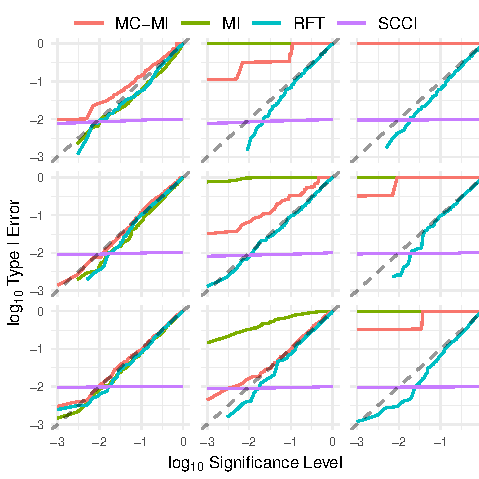
\includegraphics[scale=0.8]{imgs/calibration_add_vars.pdf}
		\caption{Type I error vs significance level for sample sizes (top to
		bottom): $ [20, 40, 80] $ and number of conditional variables (left to
		right): $ [1, 3, 5] $ on conditionally independent simulated binary
		datasets.}
	\end{figure}
\end{frame}

\begin{frame}
	\frametitle{Empirical Analysis: Discrimination}
	\begin{figure}
		\centering
		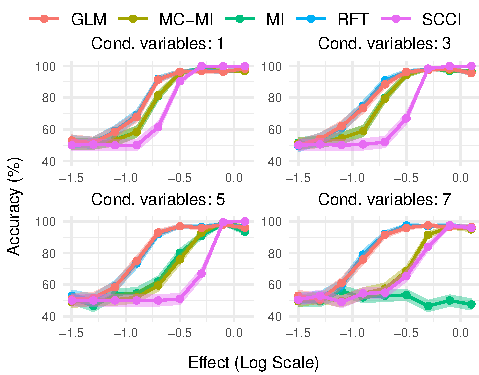
\includegraphics{imgs/accuracy.pdf}
		\caption{Accuracy (shading: mean $\pm$ standard error, $N=200$)
		of classifying simulated binary datasets (sample size: $1000$)
		as conditionally dependent or independent.}
	\end{figure}
\end{frame}

\begin{frame}
	\frametitle{Empirical Analysis: Discrimination}
	\begin{figure}
		\centering
		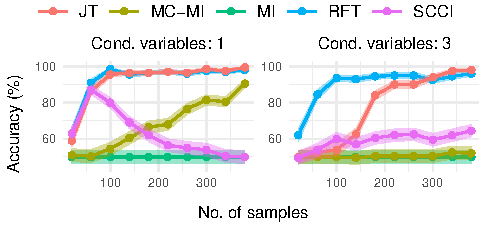
\includegraphics{imgs/accuracy_ordinal.pdf}
		\caption{Accuracy (shading: mean $\pm$ standard error) of
		classifying simulated ordinal data (8 levels per variable) as
		conditionally dependent or independent.}	
	\end{figure}
\end{frame}

\begin{frame}
	\frametitle{Applications: Model testing}
	\begin{figure}
		\centering
		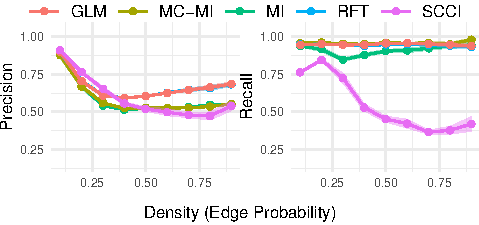
\includegraphics{imgs/model_testing.pdf}
		\caption{Precision and recall (shading: mean $\pm$ standard
		error) of testing implied CIs and equal number of randomly
		generated CIs in binary datasets (sample size: $1000$)
		simulated from random DAGs on $ 20 $ variables.}
	\end{figure}
\end{frame}

\begin{frame}
	\frametitle{Applications: Structure Learning}
	\begin{figure}
		\centering
		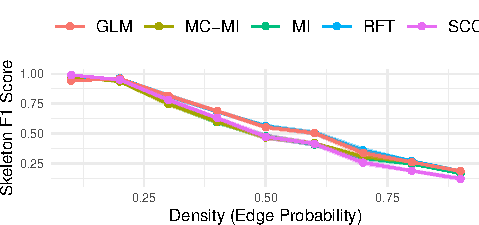
\includegraphics{imgs/sl_density.pdf}
		\caption{Structure learning on simulated data. F1-score
		(shading: mean $\pm$ standard error) of the learned model
		skeletons for randomly generated DAGs with $20$ variables and
		varying edge probabilities.  Binary datasets of $ 1000 $
		samples are simulated from the DAGs using logistic models with
		all coefficients set to $ 0.15$. Presence of an edge is
		considered the "positive" case for computing the F1-Scores.}
	\end{figure}
\end{frame}

\begin{frame}
	\frametitle{Applications: Structure Learning}
	\begin{figure}
		\centering
		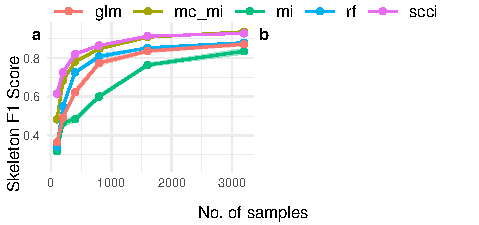
\includegraphics{imgs/sl.pdf}
		\caption{Structure learning on (a) ``alarm'', and (b)
		``insurance'' datasets.  F1-score (shading: mean $\pm$ standard
		error, $N=10$) of the learned model skeletons.  Presence of an
		edge is considered the "positive" case for computing the
		F1-Scores.}
	\end{figure}
\end{frame}

\begin{frame}
	\frametitle{Applications: Structure Learning}
	\begin{figure}
		\centering
		\begin{subfigure}{0.3\textwidth}
			\centering
			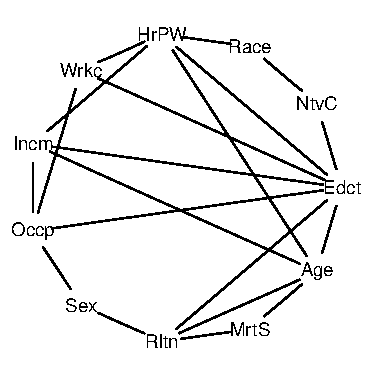
\includegraphics[scale=0.85]{imgs/sl-adult-rf.pdf}
			\caption{}
			\label{fig:sl_adult_model}
		\end{subfigure}%
		\begin{subfigure}{0.2\textwidth}
			\centering
			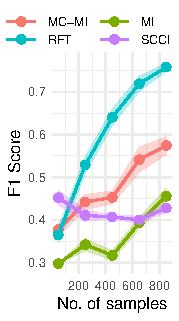
\includegraphics{imgs/adult_F1.pdf}
			\caption{}
			\label{fig:sl_adult}
		\end{subfigure}
		\caption{Structure learning on US census income dataset. (a)
		Skeleton estimated by the stable PC algorithm from the same
		data as in Figure~\ref{fig:pcerror} when using our CI test. (b)
		F1-score (shading: mean $\pm$ standard error, $N=10$) when
		comparing $d$-connected variable pairs from the CPDAG to
		correlated variable pairs in the dataset. Presence of
		d-connection/correlation is used as the positive case for
		computing the F1-Score}
	\end{figure}
\end{frame}

\begin{frame}
	\frametitle{Runtime Analysis}
	\begin{figure}
		\centering
		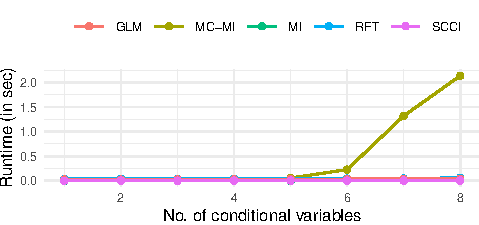
\includegraphics{imgs/runtime.pdf}
		\caption{Runtime (shading: mean $\pm$ standard error, $N=100$)
		for CI tests with varying numbers of conditional variables and
		$1000$ samples per dataset; data is generated the same way as
		in Figure~\ref{fig:cat_discrimination}.}
	\end{figure}
\end{frame}

\begin{frame}
	\frametitle{Conclusion}
	\begin{itemize}
		\item Can be extended to continuous variables.
		\item A hybrid test with mc-mi and rft.
	\end{itemize}
\end{frame}

\end{document}
